\section{Creaci�n y registro de pedidos}
En este componente se agrupan las clases que entran en juego al momento de crear un nuevo pedido.

La clase GeneradorDePedidos sirve de punto de entrada a este componente. El mismo posee el m�todo generarPedido, que es invocado por el Coordinador de pedidos, a fin de que se ingrese al sistema un nuevo pedido.

El Generador se encarga de llamar al controladorDeStock para que verifique que el stock existente sea capaz de satisfacer al pedido. Ademas el generador realiza el decremento del stock, y se encarga de realizar el callback a la gui en caso de que un insumo quede por debajo de su stock critico. %TODO: callback como?
El controlador de stock no es una clase abstracta porque creemos que no es probable que cambie su funcionamiento, el cual es bastante concreo, es decir revisar los elementos necesarios para armar los productos propios de un pedido y decrementar el stock. 

Luego de que se regisr� el decremento de stock, el Generador se encarga de llamar al EstimadorDeTiempos. Esta clase es abstracta, ya que pensamos que como la pizzeria desea ir refinando estas estimaciones, es probable que la forma de estimar se modifique de forma periodica. Por lo tanto, decidimos aplicar el \textit{Strategy pattern} a fin de poder lograr varias estrategias de estimaci�n. La Estimaci�n desarrollada en \ref{modifEstim} es implementada por la clase EstimadorBasico.

\textcolor{Red}{TODO: interacciones de estas clases con la GUI}

\textcolor{Red}{TODO: explicacion de metodos importantes}
\subsection{Modelado de escenarios}

\subsubsection{Creacion de un pedido}
Cuando el coordinador de pedidos recibe la orden de crear un nuevo pedido, la deriva al generador de pedidos. Este se encargar� de devolverle un pedido nuevo. El generador de pedidos invoca al controlador del stock, para que verifique la factibilidad de ingresar el pedido, en caso de no ser posible el generador producira una excepcion que sera propagada para porder mostrar que producto no pudo satisfacerse.

En este escenario modelaremos el proceso de creaci�n de una forma general, en particular para un pedido de mostrador, para luego mostrar escenarios particulares que pueden ocurrir durante este proceso.

En primer lugar el generador invoca al controlador de stock para que realice el chequeo y en caso de ser posible decremente el sotck. 

Luego se genera un ID para el pedido y se lo crea. Una vez creado el pedido, este pasa al asignador de horno que establece que horno le corresponde al pedido (en caso de que corresponda). Luego se procede a realizar la estimaci�n de tiempos de cocci�n. Finalmente el pedido queda ingresado

El diagrama de secuencias es el siguiente:

\begin{figure}[H]
\centering
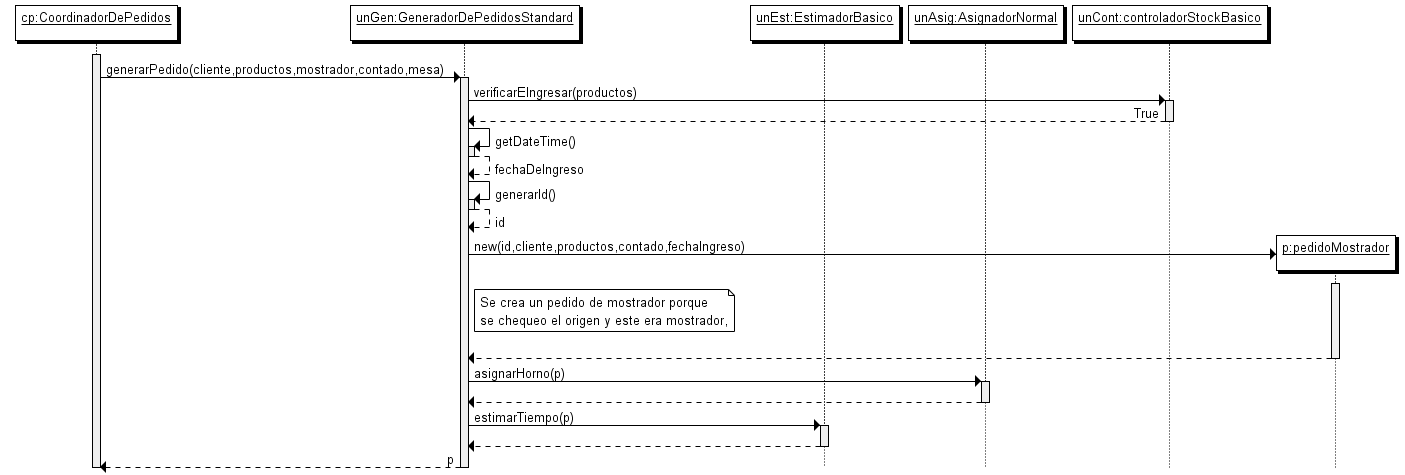
\includegraphics[height=9cm]{./figuras/crearMostrador.png}
\caption{Creaci�n de un nuevo pedido}
\end{figure}

\subsubsection{Estimacion de tiempos}

\subsubsection{Verificaci�n de stock}
El verificador de stock tiene por responsabilidad controlar que solo ingresen pedidos que puedan ser satisfechos. Ademas en caso de ser necesario debera notificar la existencia de insumos en stock critico.

Como vimos en el escenario anterior, el generador invoca el metodo verificarEIngresar. Este metodo va a intentar decrementar el stock de los insumos de cada producto del pedido que se desea armar. Para eso va a decrementar el stock siempre que sea posible, guardando aquellos productos cuyos insumos ya modifico para poder hacer rollback en caso de que el pedido no se pueda satisfacer. Si ocurre que hay un insumo de un producto cuyo insumo es insuficiente, se procede a restablecer el stock ya decrementado y luego se genera un excepcion que permite que se pueda mostrar en pantalla cual fue el pedido que genero el error al intentar ingresar.

En cambio si todos los productos se pudieron ingresar, la funci�n retorna True para indicar que termino exitosamente.

\begin{figure}[H]
\centering
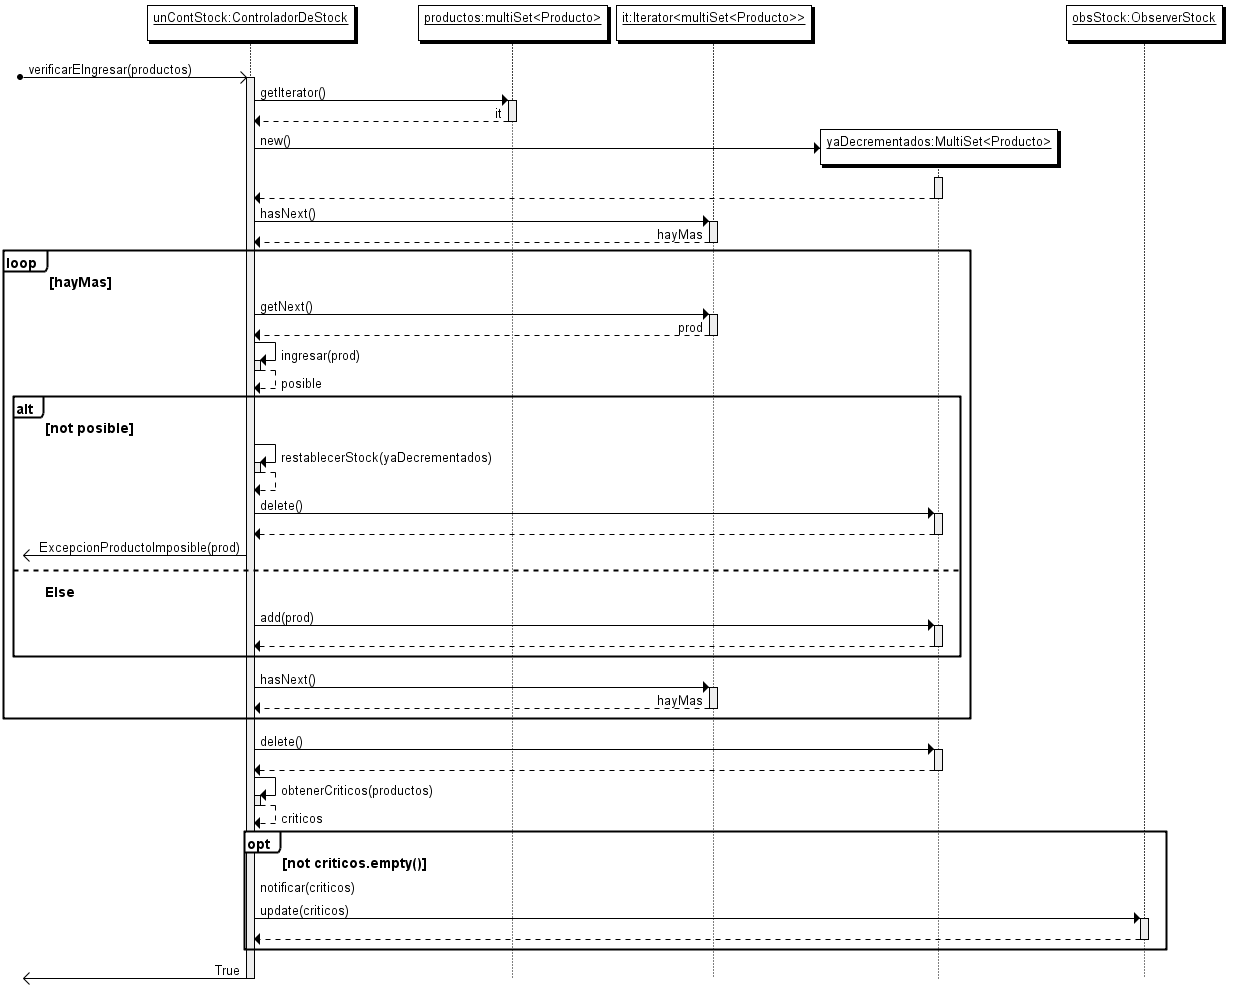
\includegraphics[height=15cm]{./figuras/verificarEIngresar.png}
\caption{Verificaci�n y decremento de stock de los insumos}
\end{figure}

Decidimos factorizar el diagrama de modo que algunas interacciones las mostraremos a continuaci�n. El metodo ingresar realiza la verificaci�n pero a nivel de cada producto, es decir revisa dado un producto que exista una cantidad de insumos necesaria. Al igual que el metodo anterior va recordando los stocks que ya modifico para hacer rollback en caso de que sea necesario.

\begin{figure}[H]
\centering
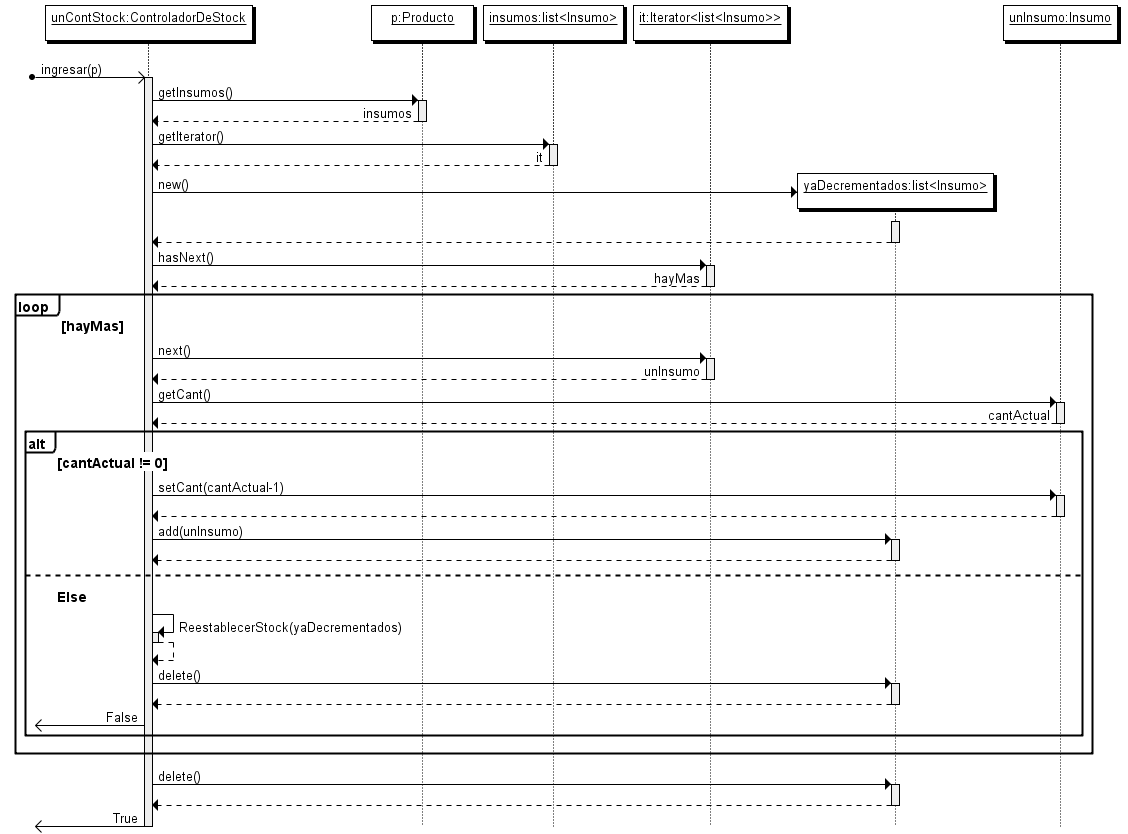
\includegraphics[height=11cm]{./figuras/ingresar(ControladorStock)}
\caption{Verificaci�n y decremento de stock de los insumos}
\end{figure}

Hay dos metodos restablecerStock, uno trabaja sobre productos y otro a nivel de insumos. El primero recorre los productos llamando al segundo para los insumos de cada producto que itera. Mientras que a nivel de insumos, lo que se hace es incrementar la cantidad de cada insumo que aparece en la lista. Como dijimos anteriormente, estos metodos permiten realizar un rollback para dehacer los cambios hechos en el stock en el caso de que la operaci�n de ingreso no sea exitosa

\begin{figure}[H]
\centering
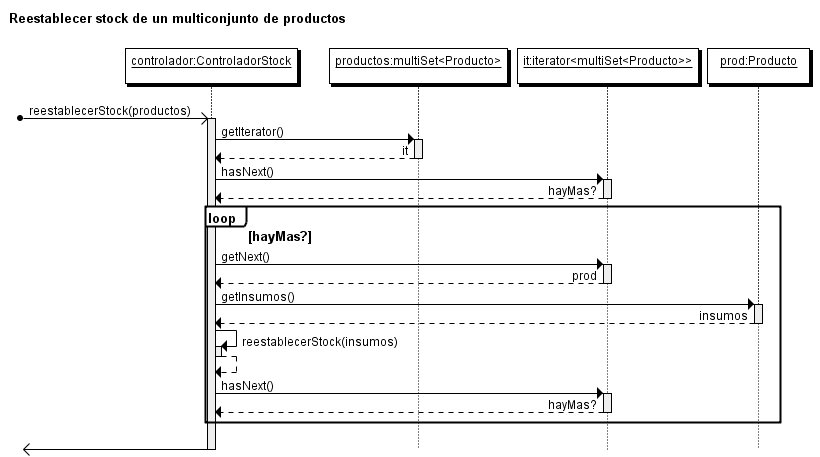
\includegraphics[height=9cm]{./figuras/reestablecerStockProductos}
\caption{restableciendo el stock de los productos cuyo }
\end{figure}

\begin{figure}[H]
\centering
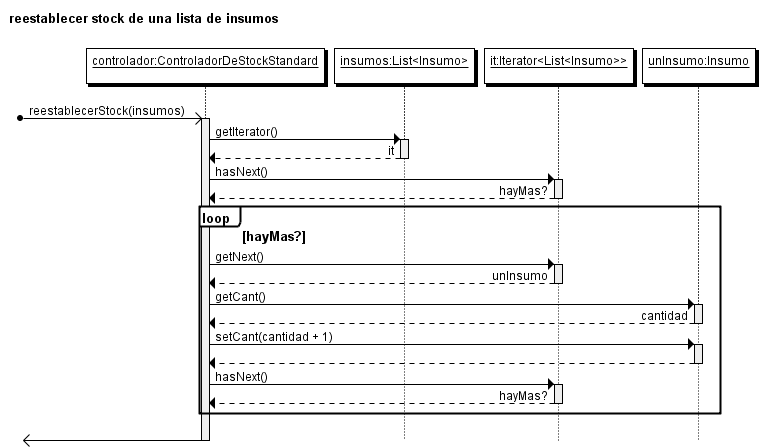
\includegraphics[height=9cm]{./figuras/reestablecerStockInsumos}
\caption{restableciendo el stock de los productos cuyo }
\end{figure}

{\color{purple}
\subsubsection{asignar horno}
\begin{itemize}
\item asignacion automatica
\item asignacion manual
\end{itemize}
}
\subsubsection{Estimacion de tiempos}

\textcolor{Red}{TODO: pseudocodigos que muestren algoritmos como por ej estimacion de tiempos}